\documentclass[runningheads]{llncs}

\usepackage[T1]{fontenc}
\usepackage{graphicx}
\usepackage{amsmath}
\usepackage{booktabs}
\usepackage{url}

\begin{document}

\title{A Reproducible Multi-View Mammogram Classification Baseline Using Dual-View Fusion on VinDr-Mammo}

\titlerunning{Reproducible Multi-View Mammogram Classification}

\author{Jitendra Sai Kota\inst{1} \and
Saddam Hossain Irfan\inst{1} \and
Muhammad Imran\inst{1}}

\authorrunning{J.S. Kota et al.}

\institute{School of Data Science and Analytics, Kennesaw State University,
Marietta, GA 30060, USA}

\maketitle

\begin{abstract}
Mammogram classification systems are often difficult to compare because studies use different label definitions, image preprocessing steps, data splits, and evaluation rules. This lack of agreement makes it hard to judge whether a new model is truly better or only benefits from a different experimental setup. This paper presents a clear and reproducible baseline for breast-level mammogram classification on the VinDr-Mammo dataset. The study focuses on a practical clinical question: whether a breast should be treated as routine or should receive further attention. We map BI-RADS 1 and 2 to the routine class and BI-RADS 3, 4, and 5 to the attention class. We compare single-view classification with a dual-view model that uses both craniocaudal (CC) and mediolateral oblique (MLO) views of the same breast. The model uses a shared EfficientNet-B5 backbone and averages the learned CC and MLO embeddings before classification. We also test three contrastive learning objectives. Across five study-level cross-validation folds, dual-view fusion improves mean AUC from 0.784 to 0.795 and improves mean F1-score from 0.432 to 0.456. Contrastive losses give small AUC changes but no consistent practical gain. The implementation is publicly available at https://github.com/iCARE-Lab/vindr-mammo-dual-view-classification.

\keywords{Mammography \and Multi-view classification \and Reproducible machine learning \and EfficientNet-B5 \and VinDr-Mammo \and BI-RADS \and Medical AI}
\end{abstract}

\section{Introduction}
\label{sec:introduction}

Breast cancer remains one of the most common cancers worldwide. In 2022, about 2.3 million new cases and 670,000 deaths were reported~\cite{iarc2022breast}. Mammographic screening is still one of the main tools for early detection. When breast cancer is found at a localized stage, the five-year survival rate is above 99\%~\cite{seer2024breast}. For this reason, reliable screening tools matter greatly for both patients and health systems.

Deep learning has become an important part of computer-aided detection and diagnosis for mammography~\cite{andreadis2025cad}. Many published models, however, treat each mammogram image as a separate input. This is different from clinical practice. Radiologists do not usually read a single view in isolation. They compare the craniocaudal (CC) and mediolateral oblique (MLO) views, and they use the two views together to understand the breast tissue. The CC view shows the breast from above, while the MLO view shows it from an oblique angle. Each view carries useful information that may not be clear in the other view.

This gap between clinical reading and model design motivates the main question of this paper: does a simple dual-view model provide a stronger baseline than a single-view model under a controlled and reproducible experimental setup? We study this question on VinDr-Mammo~\cite{nguyen2023vindr}, a public dataset with 20,000 full-field digital mammography images from 5,000 studies. We use the same preprocessing, augmentation, training protocol, and evaluation rules across all experiments so that the effect of multi-view fusion can be studied directly.

The paper also studies contrastive learning. The idea is natural: CC and MLO images from the same breast should produce related feature representations. If a model is trained to pull these paired views closer in the feature space, it may learn better features. We test this idea through cosine similarity loss, NT-Xent loss, supervised contrastive loss, and a memory bank extension. The results show that contrastive learning does not give a consistent benefit in our setting. We explain why this happens and provide guidance for future studies.

The main contributions of this work are:
\begin{enumerate}
    \item We present a reproducible breast-level classification baseline for VinDr-Mammo using a clear BI-RADS label definition and study-level cross-validation.
    \item We show that simple dual-view average fusion improves over single-view classification across five folds.
    \item We test multiple contrastive learning objectives and explain why they do not provide stable gains under strong class imbalance and small positive sample counts.
    \item We report practical ablations on resizing and augmentation choices for full-field mammogram classification.
\end{enumerate}

\section{Related Work}
\label{sec:related}

\subsection{Deep Learning for Mammogram Classification}

Early deep learning work in mammography often used small image patches or pre-selected lesion regions~\cite{shen2019deep}. More recent work has moved toward full-field mammogram classification. Several studies have compared general deep learning backbones and mammography-specific designs~\cite{sharma2025comparative}. EfficientNet~\cite{tan2019efficientnet} is often a strong backbone because it balances model size and accuracy through compound scaling. For this reason, we use EfficientNet-B5 as a stable baseline backbone.

\subsection{Multi-View Mammogram Analysis}

Multi-view learning is important because mammography exams are naturally multi-view. Sun et al.~\cite{sun2022multiview} used a multi-view convolutional neural network with an inter-view consistency term. Sarker et al.~\cite{sarker2024mvswint} proposed MV-Swin-T, a transformer-based model for multi-view mammogram classification on VinDr-Mammo. That work reports high AUC, but several independent attempts have reported much lower values of approximately 0.64, suggesting that some preprocessing or implementation details may be hard to reproduce. While the exact cause is unknown without access to their dataset loading code, one plausible explanation is image-level rather than study-level splitting, which would allow the same patient to appear in both training and test sets and inflate reported AUC. Kebede et al.~\cite{kebede2024dual} studied dual-view breast abnormality classification on VinDr-Mammo using five-fold cross-validation and reported an AUC of 0.83, which is closer to our results. Yoshitsugu et al.~\cite{yoshitsugu2026roi} studied ROI-stratified classification on VinDr-Mammo, but their reported metrics do not include AUC.

\subsection{Contrastive Learning}

Contrastive learning trains models by pulling related samples closer together and pushing unrelated samples apart. SimCLR~\cite{chen2020simclr} introduced the NT-Xent loss for self-supervised representation learning. Supervised contrastive learning~\cite{khosla2020supcon} extends this idea using class labels. MoCo~\cite{he2020moco} uses a memory bank to increase the number of negative examples. In medical imaging, contrastive learning has been used for chest X-rays and histopathology, but its value for full-field mammogram classification is less clear.

\section{Methodology}
\label{sec:method}

\subsection{Dataset and Label Definition}

We use the VinDr-Mammo dataset~\cite{nguyen2023vindr}, which contains 20,000 full-field digital mammography images from 5,000 studies. The official split contains 16,000 training images and 4,000 test images. We define each breast as one sample using the tuple (study\_id, laterality). We map BI-RADS 1 and 2 to class 0 (routine) and BI-RADS 3, 4, and 5 to class 1 (needs attention). This grouping reflects a practical clinical decision point and includes the ambiguous BI-RADS 3 in the positive class, making the task harder than groupings that separate only the most suspicious cases.

For dual-view experiments, we group images by (study\_id, laterality) to match CC and MLO views of the same breast. If a breast has multiple CC or MLO images, we keep the first available image for that view. This occurs infrequently in VinDr-Mammo, as most breasts have exactly one CC and one MLO image. However, supplementary views are sometimes acquired when the initial image is inadequate, and systematically retaining only the first image may introduce a mild selection bias toward standard acquisitions. This produces 8,000 training pairs and 2,000 test pairs. We use five stratified folds at the study level to prevent patient-level data leakage. Each fold has about 616 positive and 5,783 negative training pairs.

\subsection{Preprocessing}

All images follow the same preprocessing pipeline. First, Otsu thresholding is used to find the largest connected breast region and crop the black background with a 2\% margin. Second, Contrast Limited Adaptive Histogram Equalization (CLAHE) is applied with clip limit 2.0 and tile grid size $8\times8$. Third, the image is resized while preserving aspect ratio to fit inside $1024\times1024$, then zero-padded to exactly $1024\times1024$.

\subsection{Data Augmentation}

We use only augmentations that preserve diagnostic meaning. Horizontal and vertical flips are applied synchronously to the CC and MLO views of the same breast. Synchronization is necessary because asymmetric flipping would break the anatomical correspondence between views --- a horizontally flipped CC paired with an unflipped MLO would no longer represent the same breast orientation, which could introduce false training signal. Random rotations up to $\pm10^{\circ}$ are applied independently to each view. Brightness augmentation is excluded because mammogram intensity values carry information about tissue density.

\subsection{Model Architecture}

We use EfficientNet-B5~\cite{tan2019efficientnet} pretrained on ImageNet-1K~\cite{deng2009imagenet}. For the single-view baseline, the backbone is followed by global average pooling, dropout with $p=0.4$, and a linear classification head.

For the dual-view model, we use a Siamese design with shared backbone weights:
\begin{equation}
\begin{split}
\mathbf{e}_{CC} &= \text{GAP}(f_\theta(x_{CC})), \\
\mathbf{e}_{MLO} &= \text{GAP}(f_\theta(x_{MLO}))
\end{split}
\end{equation}
where $f_\theta$ is the shared EfficientNet-B5 backbone and GAP is global average pooling. During training, a projection head $g_\phi$ (Linear-BN-ReLU-Linear, 128-dim) maps each embedding to a contrastive space:
\begin{equation}
\mathbf{z}_{CC} = g_\phi(\mathbf{e}_{CC}), \quad \mathbf{z}_{MLO} = g_\phi(\mathbf{e}_{MLO})
\end{equation}
The classifier uses the average of the CC and MLO embeddings:
\begin{equation}
\hat{y} = h_\psi\!\left(\frac{\mathbf{e}_{CC} + \mathbf{e}_{MLO}}{2}\right)
\end{equation}
The projection head is removed at inference time, following SimCLR~\cite{chen2020simclr} and SupCon~\cite{khosla2020supcon}. The proposed architecture is shown in Fig.~\ref{fig:architecture}.

\begin{figure}[t]
\centering
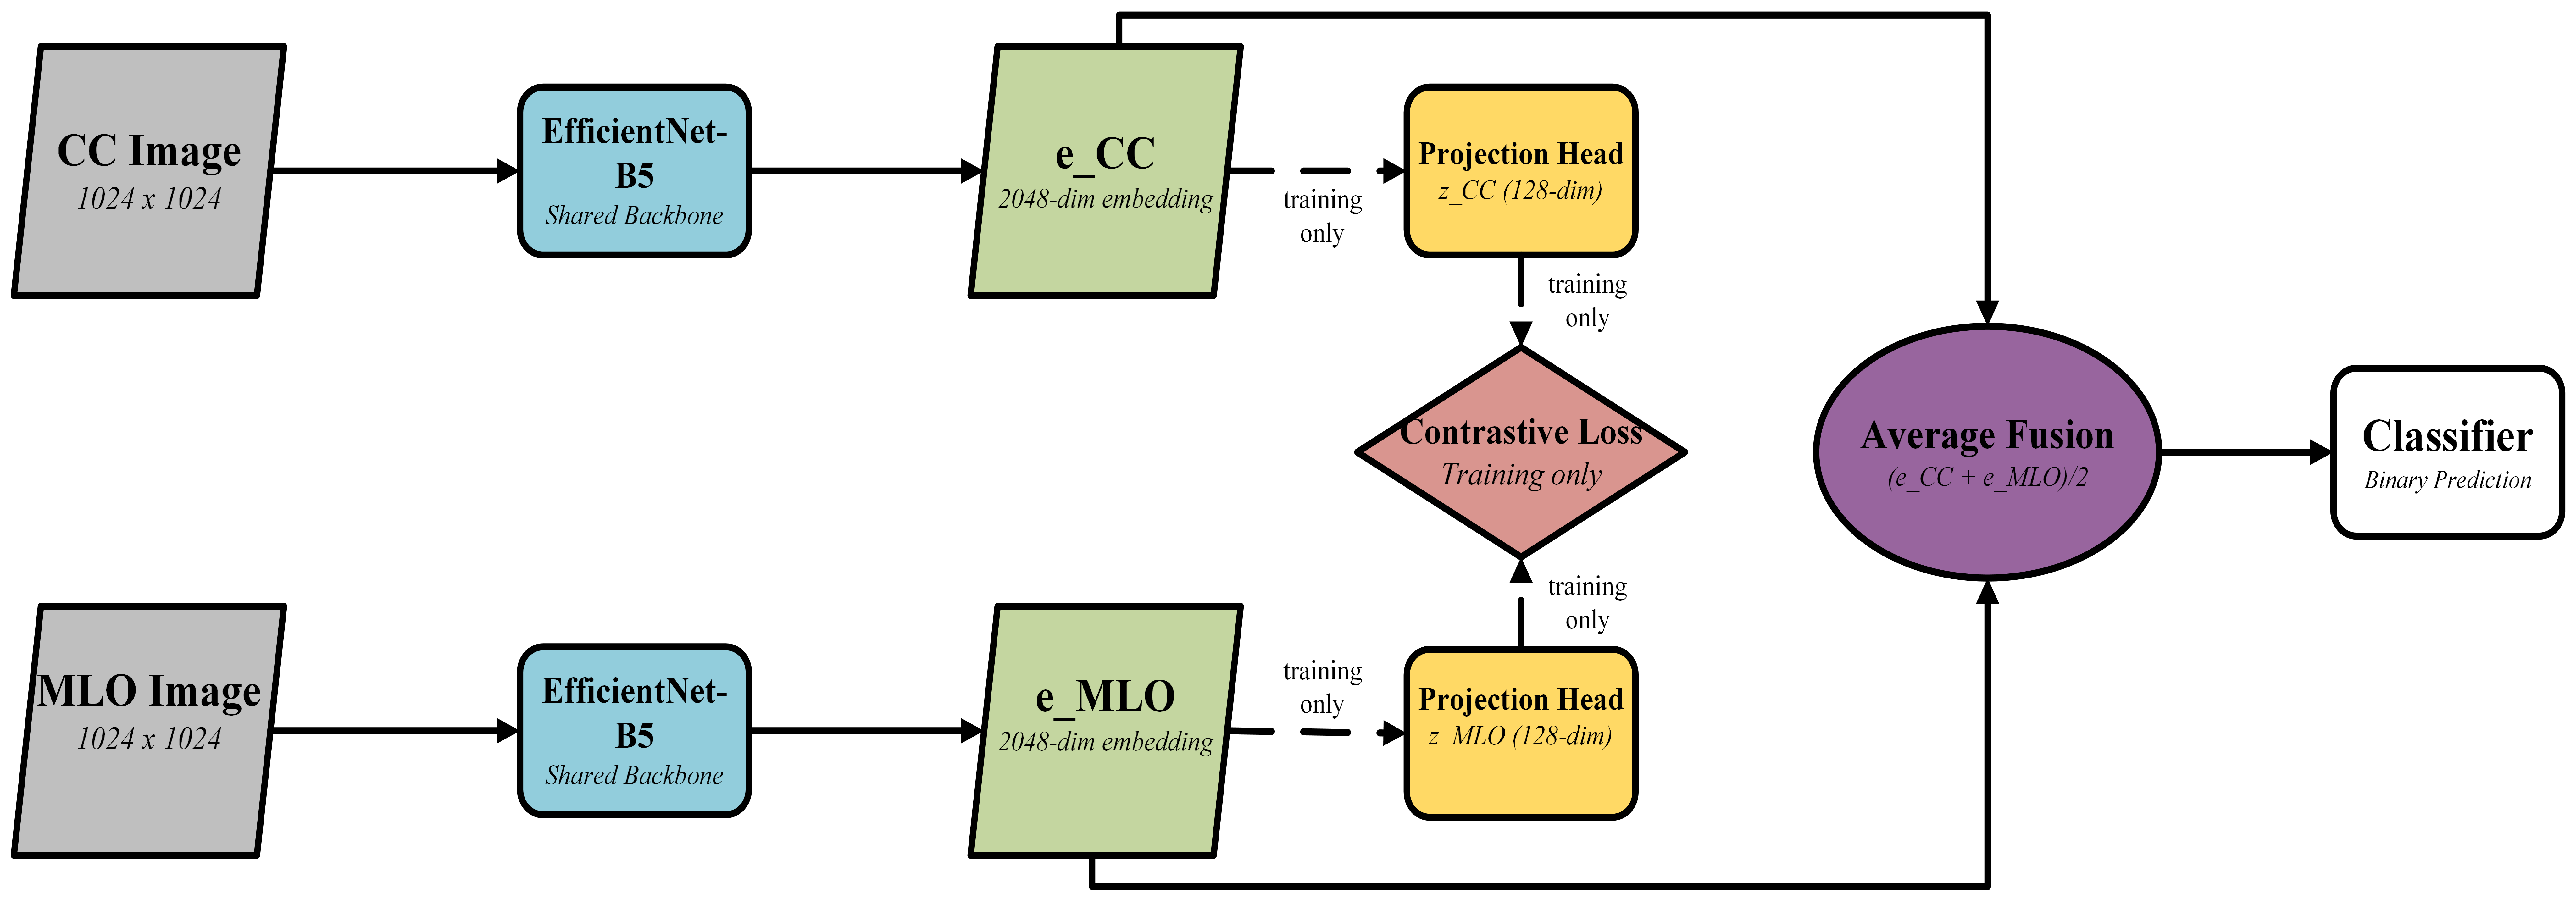
\includegraphics[width=\textwidth]{architecture-dual-view-mammography.png}
\caption{Dual-view mammogram classification architecture. CC and MLO images are processed by a shared EfficientNet-B5 backbone. The projection head is used only during training for contrastive learning. At inference, the classifier uses the average of the CC and MLO embeddings.}
\label{fig:architecture}
\end{figure}

\subsection{Contrastive Learning Objectives}

We test three contrastive objectives. \textbf{Cosine similarity loss} pulls the CC and MLO embeddings from the same breast together:
\begin{equation}
\mathcal{L}_{\text{cos}} = 1 - \frac{\mathbf{z}_{CC} \cdot \mathbf{z}_{MLO}}{\|\mathbf{z}_{CC}\|\|\mathbf{z}_{MLO}\|}
\end{equation}
\textbf{NT-Xent}~\cite{chen2020simclr} treats same-breast pairs as positives with temperature $\tau=0.07$. \textbf{Supervised contrastive loss (SupCon)}~\cite{khosla2020supcon} additionally treats same-class samples as positives:
\begin{equation}
\mathcal{L}_i = \frac{-1}{|P(i)|}\sum_{p \in P(i)} \log \frac{\exp(\mathbf{z}_i \cdot \mathbf{z}_p / \tau)}{\sum_{a \neq i} \exp(\mathbf{z}_i \cdot \mathbf{z}_a / \tau)}
\end{equation}
A \textbf{memory bank} extension~\cite{he2020moco} stores $K=512$ previous embeddings. Total training loss is:
\begin{equation}
\mathcal{L} = \mathcal{L}_{BCE} + \lambda \cdot \mathcal{L}_{con}, \quad \lambda = 0.5
\end{equation}
For numerical stability, we use a logsumexp form and \texttt{torch.where} to prevent NaN values.

\subsection{Training Protocol}

All models use differential learning rates from the first epoch: $2\times10^{-5}$ for the backbone and $2\times10^{-4}$ for the heads, with Adam optimizer and weight decay $10^{-4}$. A cosine annealing schedule lowers the learning rate to $10^{-7}$ over 200 epochs. Early stopping monitors validation AUC with patience 20. Class imbalance is handled via WeightedRandomSampler and BCEWithLogitsLoss with positive class weight $w_+ = N_{\text{neg}}/N_{\text{pos}}$. The classification threshold is selected independently for each fold using that fold's validation set by maximizing F1-score. All test metrics for that fold are computed at the fold-specific threshold. All experiments are run on one NVIDIA A100 80GB GPU using PyTorch 1.12.0 and CUDA 11.7.

\section{Results}
\label{sec:results}

\subsection{Single-View vs Multi-View Baseline}

Table~\ref{tab:sv_mv} compares the single-view and dual-view models. The dual-view model improves AUC in four of five folds. Mean AUC increases from 0.784 to 0.795 and mean F1-score from 0.432 to 0.456. We conducted a Wilcoxon signed-rank test comparing single-view and dual-view AUC across five folds. However, this test requires a minimum of six pairs to produce a reliable p-value, making the result ($p=0.156$),  statistically inconclusive at this sample size. The improvement is nonetheless consistent across four of five folds, with a mean gain of +0.011 AUC.

\begin{table}[h]
\caption{Single-view vs. dual-view average fusion on VinDr-Mammo (5-fold CV).}
\label{tab:sv_mv}
\centering
\begin{tabular}{|l|c|c|c|c|c|c|}
\hline
\textbf{Method} & \textbf{F0} & \textbf{F1} & \textbf{F2} & \textbf{F3} & \textbf{F4} & \textbf{Mean} \\
\hline
SV AUC & 0.782 & 0.784 & 0.799 & 0.790 & 0.764 & 0.784 \\
MV AUC & 0.787 & 0.804 & 0.814 & 0.774 & 0.797 & \textbf{0.795} \\
\hline
SV F1  & 0.422 & 0.451 & 0.448 & 0.444 & 0.397 & 0.432 \\
MV F1  & 0.455 & 0.478 & 0.473 & 0.427 & 0.448 & \textbf{0.456} \\
\hline
\end{tabular}
\end{table}

\subsection{Contrastive Loss Ablation}

Table~\ref{tab:contrastive} reports contrastive learning results. Cosine similarity, NT-Xent, and SupCon each reach mean AUC of 0.800, slightly above the no-contrastive model. However, gains are small and within fold-to-fold variation. The memory bank version reaches 0.797 and does not improve over the baseline. F1-score also does not improve consistently.

\begin{table}[h]
\caption{Contrastive loss ablation for the dual-view model (5-fold CV).}
\label{tab:contrastive}
\centering
\begin{tabular}{|l|c|c|c|}
\hline
\textbf{Method} & \textbf{Mean AUC} & \textbf{Std} & \textbf{Mean F1} \\
\hline
No contrastive      & 0.795 & 0.011 & 0.456 \\
Cosine similarity   & 0.800 & 0.012 & 0.451 \\
NT-Xent             & 0.800 & 0.012 & 0.409 \\
SupCon              & 0.800 & 0.016 & 0.457 \\
SupCon + MemBank    & 0.797 & 0.009 & 0.456 \\
\hline
\end{tabular}
\end{table}

\subsection{Resize Strategy Ablation}

Table~\ref{tab:resize} compares three resizing strategies. Differences are within fold-to-fold variation. We use Strategy B as default because it avoids shape distortion and works with arbitrary backbone architectures.

\begin{table}[h]
\caption{Resize strategy ablation for the dual-view model without contrastive loss (5-fold CV). AR = aspect ratio.}
\label{tab:resize}
\centering
\begin{tabular}{|l|c|c|c|}
\hline
\textbf{Strategy} & \textbf{Mean AUC} & \textbf{Std} & \textbf{Mean F1} \\
\hline
A: Squished $1024\times1024$      & 0.805 & 0.009 & 0.471 \\
B: AR + zero pad $1024\times1024$ & 0.799 & 0.013 & 0.461 \\
C: AR $614\times1024$, no pad     & 0.796 & 0.003 & 0.475 \\
\hline
\end{tabular}
\end{table}


\subsection{Contrastive Loss Weight Ablation}

Table~\ref{tab:lambda} reports the effect of the contrastive loss weight $\lambda$ on dual-view SupCon performance. Lower $\lambda$ consistently outperforms higher values, with $\lambda=0.1$ achieving the best mean AUC and F1-score. This confirms that a strong contrastive signal hurts classification when positive samples per batch are scarce.

\begin{table}[h]
\caption{Lambda ablation for the dual-view SupCon model (5-fold CV).}
\label{tab:lambda}
\centering
\begin{tabular}{|c|c|c|c|}
\hline
$\boldsymbol{\lambda}$ & \textbf{Mean AUC} & \textbf{Std} & \textbf{Mean F1} \\
\hline
0.1 & \textbf{0.811} & 0.006 & \textbf{0.464} \\
0.5 & 0.798 & 0.012 & 0.452 \\
1.0 & 0.795 & 0.018 & 0.439 \\
\hline
\end{tabular}
\end{table}

\subsection{Comparison with Related Work}

Table~\ref{tab:comparison} compares our results with related studies. Direct comparison is difficult because studies use different label groupings which strongly affect task difficulty.

\begin{table}[h]
\caption{Comparison with related work on VinDr-Mammo.}
\label{tab:comparison}
\centering
\begin{tabular}{|l|c|c|c|}
\hline
\textbf{Method} & \textbf{Positive class} & \textbf{Views} & \textbf{AUC} \\
\hline
MV-Swin-T~\cite{sarker2024mvswint}         & BI-RADS $\geq$ 4 & CC+MLO & 0.96$^*$ \\
Kebede et al.~\cite{kebede2024dual}        & Abnormality      & CC+MLO & 0.83 \\
Yoshitsugu et al.~\cite{yoshitsugu2026roi} & BI-RADS $\geq$ 2 & Single & N/A \\
\hline
Ours (Single View) & BI-RADS $\geq$ 3 & CC or MLO & 0.784 \\
Ours (Multi-View)  & BI-RADS $\geq$ 3 & CC+MLO    & \textbf{0.795} \\
\hline
\end{tabular}
\end{table}
{\small $^*$Not independently reproducible; multiple groups report $\sim$0.64.}

\section{Discussion}
\label{sec:discussion}

\subsection{Dual-View Fusion Improves the Baseline}

The results support a simple conclusion: using both CC and MLO views helps. The dual-view model improves mean AUC by 0.011 and mean F1-score by 0.024 over the single-view baseline using only average fusion, without a complex attention module or a special mammography-specific network.

\subsection{Why Contrastive Learning Does Not Give a Clear Gain}

The contrastive learning results are more mixed. We see three likely reasons. First, the batch size is only 8. With a class ratio of 9.4:1, many batches contain few or no positive samples, giving supervised contrastive loss very little positive signal. The original SupCon work used much larger batch sizes~\cite{khosla2020supcon}. Second, the positive class is visually diverse. BI-RADS 3, 4, and 5 do not all look the same, and pulling them together in the same embedding space can create conflicting training signals. Third, each fold contains only about 616 positive training pairs, which may be too small for learning stable class-level clusters.

\subsection{Label Grouping Affects Reproducibility}

The label grouping strongly affects the task. Our grouping (BI-RADS 1+2 versus 3+4+5) is clinically meaningful but harder than grouping 1+2+3 versus 4+5. Papers on VinDr-Mammo should report their label grouping clearly, as different groupings are not directly comparable.

\subsection{Implications for Software Engineering of Medical AI}

For a software-engineering audience, the main lesson is that reproducibility is a design choice. A medical AI pipeline is not only a model. It also includes image cropping, contrast enhancement, resizing, augmentation, label mapping, patient-level splitting, threshold selection, and reporting rules. Small changes in any of these steps can change the final score. This work treats the pipeline as an engineered system and intentionally keeps the model simple so that each step can be audited and repeated.

\subsection{Limitations}

This study has several limitations. First, all experiments use ImageNet-pretrained EfficientNet-B5 rather than mammography-specific pretraining. Second, the strong class imbalance gives only about 151 positive validation samples per fold, which can make validation AUC noisy. Third, the contrastive learning experiments use small batches because of GPU memory limits. Fourth, this study does not test attention-augmented architectures such as CBAM~\cite{woo2018cbam}, FCCS~\cite{maurya2024fccs}, or MLSE~\cite{xie2026mlse} in the dual-view setting.

\section{Conclusion}
\label{sec:conclusion}

This paper presents a reproducible baseline for breast-level mammogram classification on VinDr-Mammo. Under a fixed experimental setup, a simple dual-view model that averages CC and MLO embeddings improves over a single-view model, increasing mean AUC from 0.784 to 0.795 and mean F1-score from 0.432 to 0.456. Contrastive learning does not give a stable practical gain under the current class imbalance and batch-size limits. More broadly, the paper shows that careful pipeline design and transparent reporting are essential for building trustworthy medical AI systems.

\begin{credits}
\subsubsection{\ackname}
The authors thank the Kennesaw State University High Performance Computing cluster for computational resources.

\subsubsection{\discintname}
The authors have no competing interests to declare that are relevant to the content of this article.
\end{credits}

\begin{thebibliography}{99}

\bibitem{iarc2022breast}
IARC: Global Cancer Observatory: Cancer Today (2022)

\bibitem{seer2024breast}
National Cancer Institute: Cancer of the Breast (Female) --- Cancer Stat Facts. \url{https://seer.cancer.gov/statfacts/html/breast.html} (2024)

\bibitem{andreadis2025cad}
Andreadis, T., Gasteratos, A., Seimenis, I., Koulouriotis, D.: Application of CAD Systems in Breast Cancer Diagnosis Using Machine Learning Techniques: An Overview of Systematic Reviews. Bioengineering \textbf{12}(11), 1160 (2025). \url{https://doi.org/10.3390/bioengineering12111160}

\bibitem{nguyen2023vindr}
Nguyen, H.T., et al.: VinDr-Mammo: A large-scale benchmark dataset for computer-aided diagnosis in full-field digital mammography. Sci. Data \textbf{10}, 277 (2023)

\bibitem{shen2019deep}
Shen, L., et al.: Deep learning to improve breast cancer detection on screening mammography. Sci. Rep. \textbf{9}, 12495 (2019)


\bibitem{sharma2025comparative}
Sharma, S., Singh, Y., Choudhury, T.: Advanced deep learning architectures for enhanced mammography classification: a comparative study of CNNs and ViT. Discover Artif. Intell. \textbf{5}(1), 187 (2025)

\bibitem{tan2019efficientnet}
Tan, M., Le, Q.: EfficientNet: Rethinking model scaling for convolutional neural networks. In: ICML (2019)

\bibitem{sun2022multiview}
Sun, L., et al.: Breast mass classification based on supervised contrastive learning and multi-view consistency. IET Biom. Eng. (2022)

\bibitem{sarker2024mvswint}
Sarker, S., et al.: MV-Swin-T: Mammogram classification with multi-view Swin Transformer. In: ISBI (2024)

\bibitem{kebede2024dual}
Kebede, T.W., et al.: Dual-view deep learning for improved diagnosis of breast abnormalities. Sci. Rep. (2024)

\bibitem{yoshitsugu2026roi}
Yoshitsugu, K., et al.: Improving Normal/Abnormal and Benign/Malignant Classifications in Mammography with ROI-Stratified Deep Learning. Bioengineering \textbf{13}(2), 206 (2026)

\bibitem{chen2020simclr}
Chen, T., et al.: A simple framework for contrastive learning of visual representations. In: ICML (2020)

\bibitem{khosla2020supcon}
Khosla, P., et al.: Supervised contrastive learning. In: NeurIPS (2020)

\bibitem{he2020moco}
He, K., et al.: Momentum contrast for unsupervised visual representation learning. In: CVPR (2020)

\bibitem{deng2009imagenet}
Deng, J., et al.: ImageNet: A large-scale hierarchical image database. In: CVPR (2009)

\bibitem{woo2018cbam}
Woo, S., et al.: CBAM: Convolutional block attention module. In: ECCV (2018)

\bibitem{maurya2024fccs}
Maurya, R., et al.: FCCS-Net: Breast cancer classification using Multi-Level fully Convolutional-Channel and spatial attention-based transfer learning. Biomed. Signal Process. Control \textbf{94}, 106258 (2024)

\bibitem{xie2026mlse}
Xie, W., et al.: MLSE-FML: Mammogram classification with multi-level semantic extraction and focal margin loss. Biomed. Signal Process. Control \textbf{112}, 108554 (2026)

\end{thebibliography}

\end{document}
